\section[Electromagnetic calorimeters] {Electromagnetic calorimeters \label{sec:calorimeters}}

\subsection[Barrel calorimeter ]{Barrel calorimeter \label{sec:bcal}}
The barrel calorimeter (BCAL) is an electromagnetic sampling calorimeter that detects photon showers with energies between 0.05~GeV and several GeV, $11^{\circ}$--$126^{\circ}$ in polar angle, and $0^{\circ}$--$360^{\circ}$ in azimuthal angle, which defines a geometry that is fairly unique among calorimeters. The containment of showers depends on the angle of photon incidence, with a thickness of $15.3$ radiation lengths for particles entering normal to the calorimeter face and reaching up to 67 radiation lengths at $14^{\circ}$. Details of the design, construction and performance of the BCAL can be found in Ref.\cite{BEATTIE201824}.

The BCAL is constructed as a lead and  scintillating-fiber matrix, consisting of 0.5~mm-thick grooved lead sheets and 1.0~mm-diameter Kuraray SCSF-78MJ multi-clad fibers, the latter running parallel to the cylindrical axis of the detector. Each module has approximately 185 layers and 15,000 fibers. Geometrically, the BCAL consists of 48 optically isolated modules each with a trapezoidal cross section, forming a  390~cm-long cylindrical shell having inner and outer radii of 65~cm and 90~cm, respectively. The light generated in the fibers is collected via small light guides at each end of the module and transported to silicon photomultipliers (SiPMs), which were chosen due to their insensitivity to magnetic fields. The end of the calorimeter with light guides, light sensors and electronics is shown in  Fig.\,\ref{fig:bcal:bcal_assemblies}.

\begin{figure}[tbp]\centering
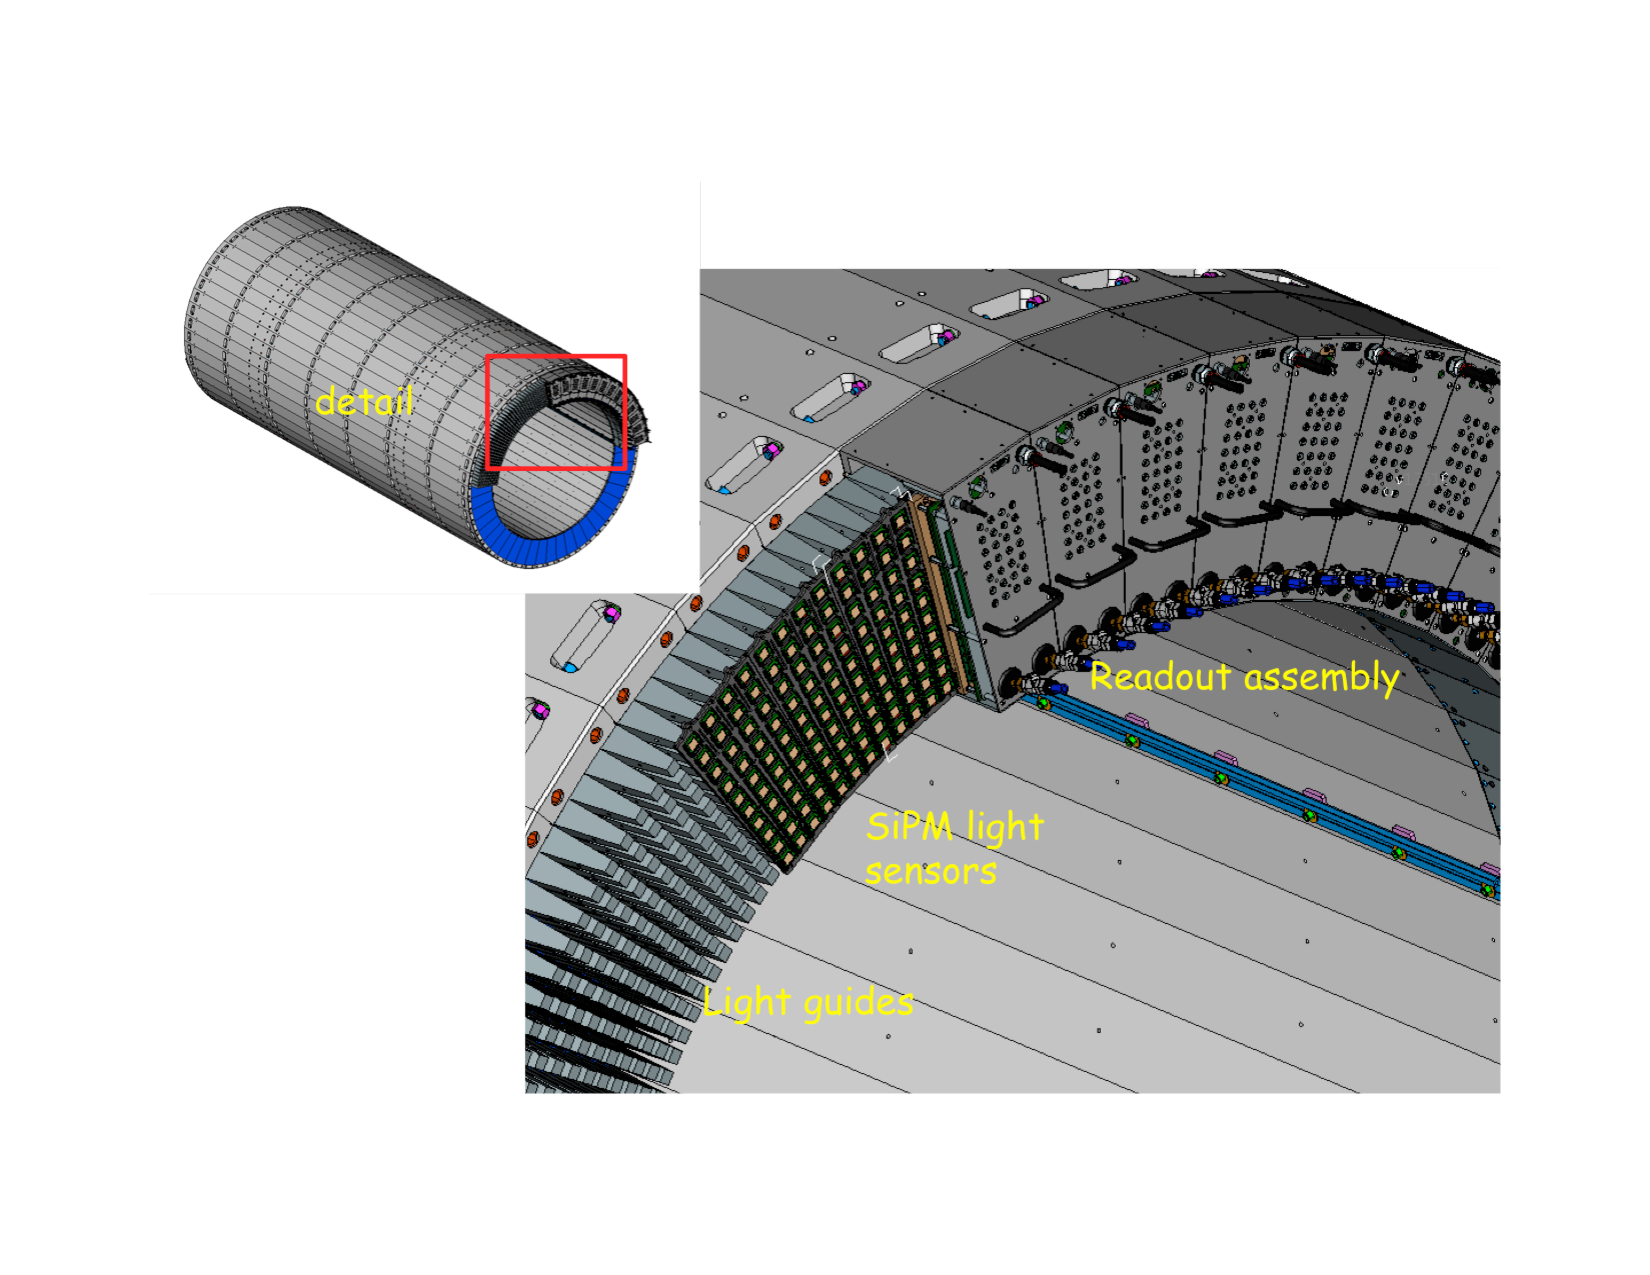
\includegraphics[scale=0.4]{figures/bcal_assemblies.pdf}
\caption{\label{fig:bcal:bcal_assemblies}
   Three-dimensional rendition of the light guides mounted at the end of the 
   BCAL, as well as the readout assemblies mounted over them. The 
   readout assemblies contain the 
   SiPMs and their electronics.  (Color online)
  }
\end{figure}


The SiPM light sensors are Hamamatsu S12045(X) Multi-Pixel Photon Counter (MPPC) arrays \footnote{Hamamatsu Corporation, Bridgewater, NJ 08807, USA \\ (\url{http://sales.hamamatsu.com/en/home.php)}.}, 
which are $4\times4$ arrays of $3\times3$ mm$^2$ tiles \cite{hdnote2913}. The SiPMs were tested extensively before acceptance \cite{Barbosa2012100,Qiang2013234,soto,Soto201489,BeattieIEEE,doi:10.1063/1.4955340}. Four thousand units were purchased and 3840 are installed in the detector. The gain of the SiPM depends on the voltage above the breakdown voltage, which is about 70~V. We operate them at 1.4~V over the breakdown voltage, which was selected to reduce the effect of readout thresholds. Even at this relatively high over-bias, the noise level is dominated by fluctuations in the electronics baseline and not by single-pixel noise. In order to keep a constant gain, we maintained the temperature within practical limits ($\pm$ 2$^\circ$C) using a chilled water system and then stabilized the gain using a custom circuit that adjusted the bias voltage based on the measured temperature. Two stages of preamplifiers and summing electronics are attached to the sensors. In order to reduce the number of signals that are digitized, circuits sum the outputs of the preamplifiers in groups of radial columns, with coarser granularity away from the target. The layer closest to the target consists of a single SiPM, and the next three have 2, 3, and 4 SiPMs, respectively. On the end of each module, forty SiPMs generate sixteen signals that are delivered to flash ADCs (FADCs) and twelve signals that are discriminated and then recorded with pipeline TDCs. The FADCs and TDCs are conveniently located on the floor of the experimental hall in VXS crates.

\begin{figure}[tbp]\centering
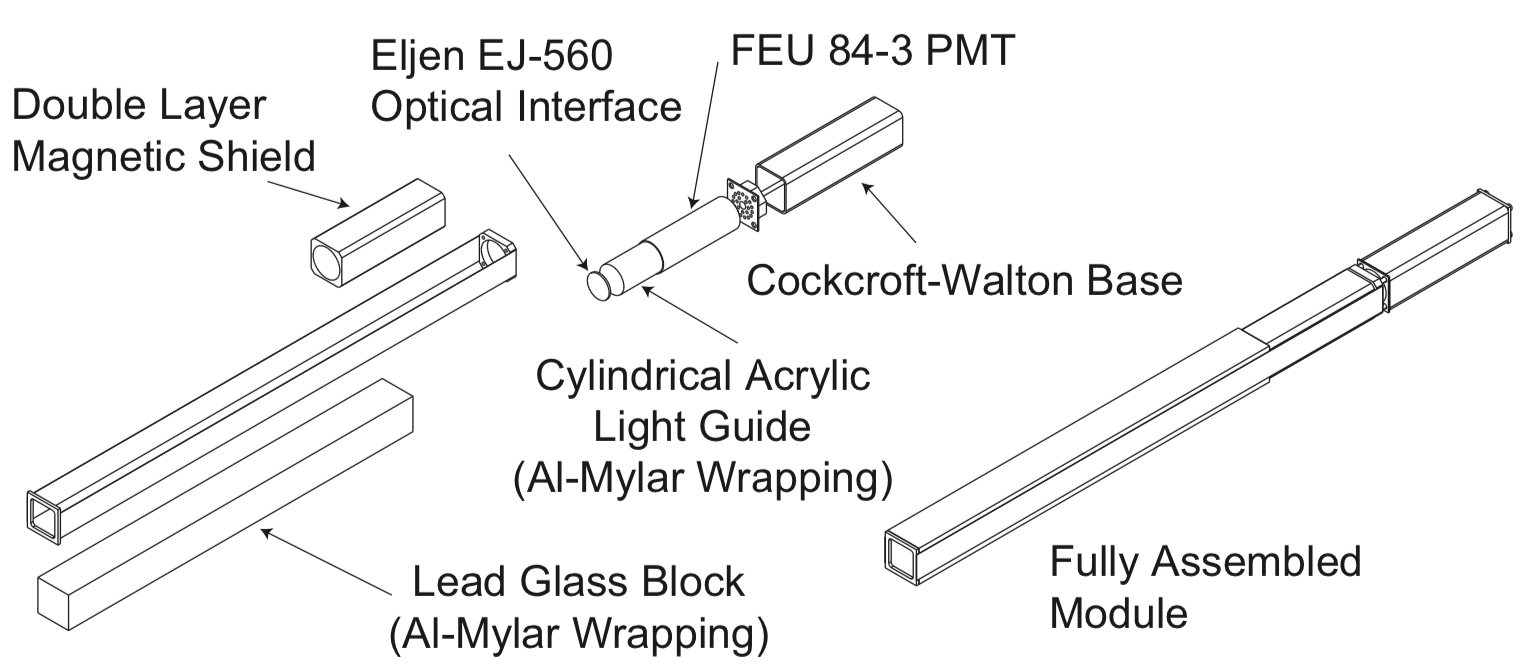
\includegraphics[height=5cm]{figures/FCAL_single_module}
\caption{\label{fig:fcal:FCAL_single_module}
    Expanded view of a single FCAL module.
  }
\end{figure} 
\subsection{Forward calorimeter \label{sec:fcal}}
The forward calorimeter (FCAL) detects photon showers with energies ranging from 0.1 GeV to several GeV, and  between $1^{\circ}$--$11^{\circ}$ in polar angle. The FCAL is located 5.6~m downstream from the center of the GlueX target and consists of 2800 lead glass blocks --- each having transverse dimensions $4\times4$ cm$^2$ and length of 45~cm ---  stacked in a circular array that has a diameter of 2.4~m.  The lead glass blocks are equivalent to type F8 manufactured by the Lytkarino Optical Glass Factory,\footnote{http://lzos.ru .}. The blocks and most of the PMTs are the same as those used in previous experiments: E852 at Brookhaven National Laboratory \cite{CRITTENDEN1997377} and the RadPhi Experiment at JLab \cite{JONES2007384}. The glass was annealed by heat treatment prior to installation in GlueX. The detector is enclosed in a dark room.

The light collection from the lead-glass block into the PMT is accomplished, sequentially, via an Eljen EJ-560 optical interface ``cookie'' and an acrylic cylindrical light guide glued to the PMT. The light guide recesses the magnetically sensitive photocathode of the PMT inside a dual layer of soft iron and mu-metal that attenuates the stray field of the GlueX solenoid of up to 200~G. The sensors are FEU 84-3 PMTs with Cockcroft-Walton bases, each consuming 0.2~W of power.  The design of the PMT base is similar to that noted in Ref.~\cite{Brunner:1998fh} and eliminates the need for a 2800-channel high-voltage power system. The bases communicate with a controller utilizing the CAN protocol \cite{wiki:CANBus}, with 100 bases on each of 28 CAN busses.  The communication allows continuous monitoring of the PMT voltages, temperatures, and current draw.
A schematic of a single FCAL module is shown in 
Fig.\,\ref{fig:fcal:FCAL_single_module} and more details may be found in Ref.\,\cite{MORIYA201360}. FCAL signals are routed to FADC electronics, situated on a platform, directly behind the FCAL dark room.

\subsection{Electronics \label{sec:calelectronics}}
Custom readout electronics for the two calorimeters are mounted in standard VXS crates and include 
JLab 12-bit 250~MHz FADCs \cite{hdnote1022}, discriminators \cite{hdnote2511} and F1 Time-to-Digital Converters (TDCs) \cite{hdnote1021}. The maximum input scale of the FADCs (4095 counts) is set to 2~V.
The FADCs sample each calorimeter channel every 4~ns and generate raw waveforms consisting of 100 samples 
 (400~ns), which are available for further processing by the firmware upon a trigger signal if there is a threshold crossing. The firmware computes several derived features of the pulse: pedestal, peak value, integral over a selected window, and time of the half-way point on the leading edge. At most one pulse is extracted from each readout window. These pulse features constitute the raw data that is nominally read out from the FADC.  Optionally, the full waveforms can be read out for diagnostic purposes and to check the firmware output against the offline emulation of the parameter extraction; this is done for less than about 1\% of the production runs.
 
We describe the feature extraction of pulses in more detail.
Pulses are identified by the first sample that exceeds a threshold, currently set to 5 (8) counts above the average pedestal for the BCAL (FCAL). These thresholds correspond to approximately 2.5 (12) MeV for the BCAL (FCAL). The integral is determined using a fixed number of samples relative to the threshold crossing, which was determined by maximizing the ratio of signal to pedestal noise.  The integration window begins one sample before the threshold time and extends to 26 (15) samples after the threshold time for the BCAL (FCAL).  Typical pedestal widths are $\sigma\sim$1.2-1.3 (0.8) counts for the BCAL (FCAL).  For the BCAL, the pedestals are determined for each channel event-by-event, appropriately scaled, and then subtracted from the peak and integral to obtain signals proportional to the energy deposited in the calorimeter, while for the FCAL, the average pedestal over a run period is determined offline for each channel and its contribution to the pulse integral is subtracted when the data are reconstructed.  %See Fig.\,\ref{fig:Plot_waveform10}.  
 The algorithm that determines the time of the pulse is pulse-height independent and therefore no time-walk correction is required for the FADC times~\cite{Bennett:2010nf}.

The outputs of the three inner layers of the BCAL are also connected leading-edge discriminators, which feed the JLab F1 TDCs. The discriminator thresholds are typically set to about 35~mV, but are adjusted
 channel by channel.  The pulse times are recorded relative to the trigger in a 12-bit word. Multiple hits may be recorded per channel per event (up to eight), but are culled at a later time by comparison to FADC times. The nominal least count is configured to 58~ps.


\subsection[Calibration and monitoring]{Calibration and monitoring \label{sec:calcalib}}
The relative gains of the calorimeters are monitored using a modular LED-driver system \cite{Anassontzis201441}. The control system is the same for both calorimeters, but the arrangement of LEDs is tailored to the geometry of each detector. In the BCAL, there is one LED inserted into each light guide, which can be used to monitor each individual SiPM and its partner at the far end of the module.
Due to geometry the illumination varies considerably from channel to channel. 
The average stability of the detector over a period of ten days is better than 1\% and the fractional root-mean-square (RMS) deviations of the mean for each SiPM during a single data from the average over the run period is typically less than 2\%.

For the FCAL, we installed four acrylic panes, each covering the upstream end of one quadrant of the FCAL. Each pane is illuminated by forty LEDs, ten violet, ten blue and twenty green. In addition to monitoring the stability of the readout, the different colors are used to study the wavelength dependence of the transmission of light though the lead glass blocks.  In particular, radiation damage to lead glass inhibits transmission at the blue end of the spectrum and tends to turn glass a brownish color~\cite{Schaefer:2011gw}.  Throughout a several-month run, in the blocks closest to the beam line, the PMT response to violet LED degraded by about 10\% while the response to the green LED is unchanged, characteristic of radiation damage.  Such damage is only evident in the first two layers of blocks surrounding the 12~cm$\times$12~cm beam hole. This damage is likely confined to the upstream end of the block and does not significantly affect the response to particle showers in the body of the glass.

\subsection{Performance \label{sec:calperformance}}
The performance of the calorimeter is summarized by its ability to measure the energy, position and timing of electromagnetic showers.

The energy resolution of each calorimeter was extracted from the measured $\pi^0$ and $\eta$ mass distributions, which yielded consistent results. 
To study the $\eta$ mass resolution, we selected events using kinematic fits to $\gamma p \rightarrow p \pi^+ \pi^- \gamma \gamma$, with $\eta\rightarrow \gamma\gamma$ and the photons having energies within 10\%.
The proton and pion tracks were used to determine the event vertex, needed to accurately reconstruct the two-photon invariant mass.
This reaction provides a fairly clean sample of $\eta$'s with energy ``symmetric" photons recorded either both in the BCAL or both in the FCAL. 
The single-photon energy resolution was determined from Gaussian fits to the $\eta$ invariant mass width, neglecting contributions from uncertainty in the opening angle.
Monte Carlo simulation of $\gamma p \rightarrow p \pi^+ \pi^- \eta$ events, with kinematics chosen to approximate the experimental distributions, were used to tune the MC resolution to match the data. 
The single-photon resolutions are shown in Fig.\,\ref{fig:bcal:eta_resolution}\,a) for the BCAL and Fig.\,\ref{fig:bcal:eta_resolution}\,b) for the FCAL as a function of the mean photon energy, both for data and simulation.
A fit has been performed to the data for each calorimeter to estimate contributions to noise from stochastic and constant processes.  The parameters in the fit are correlated due to the limited range in energy available for this data.

The position resolution ($\sim$\,2.5 cm) is determined by the timing resolution of the system, which was determined to be $\sigma=150$\,ps at 1\,GeV.


\begin{figure}[tbh]\centering
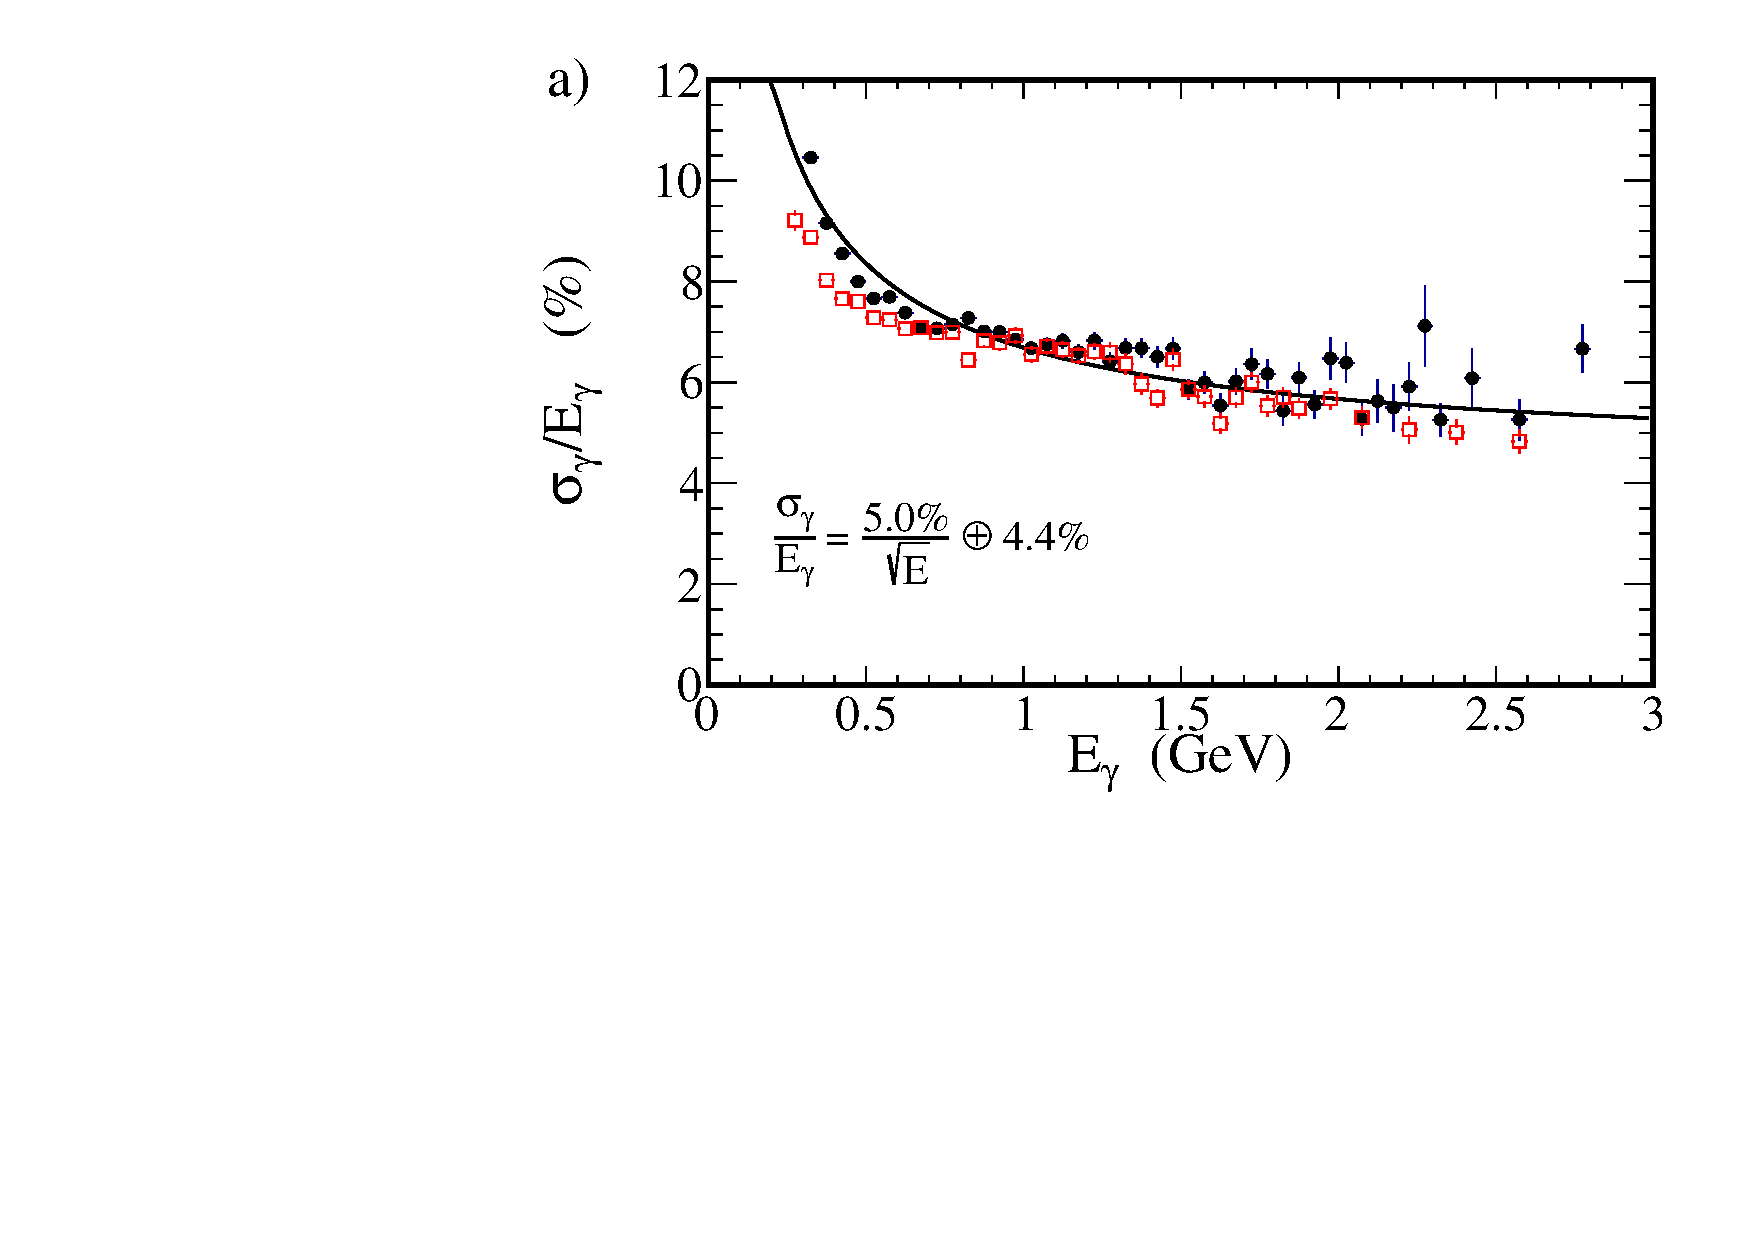
\includegraphics[width=0.48\textwidth]{figures/fit_BCAL_energy_resolution_sigma.pdf} 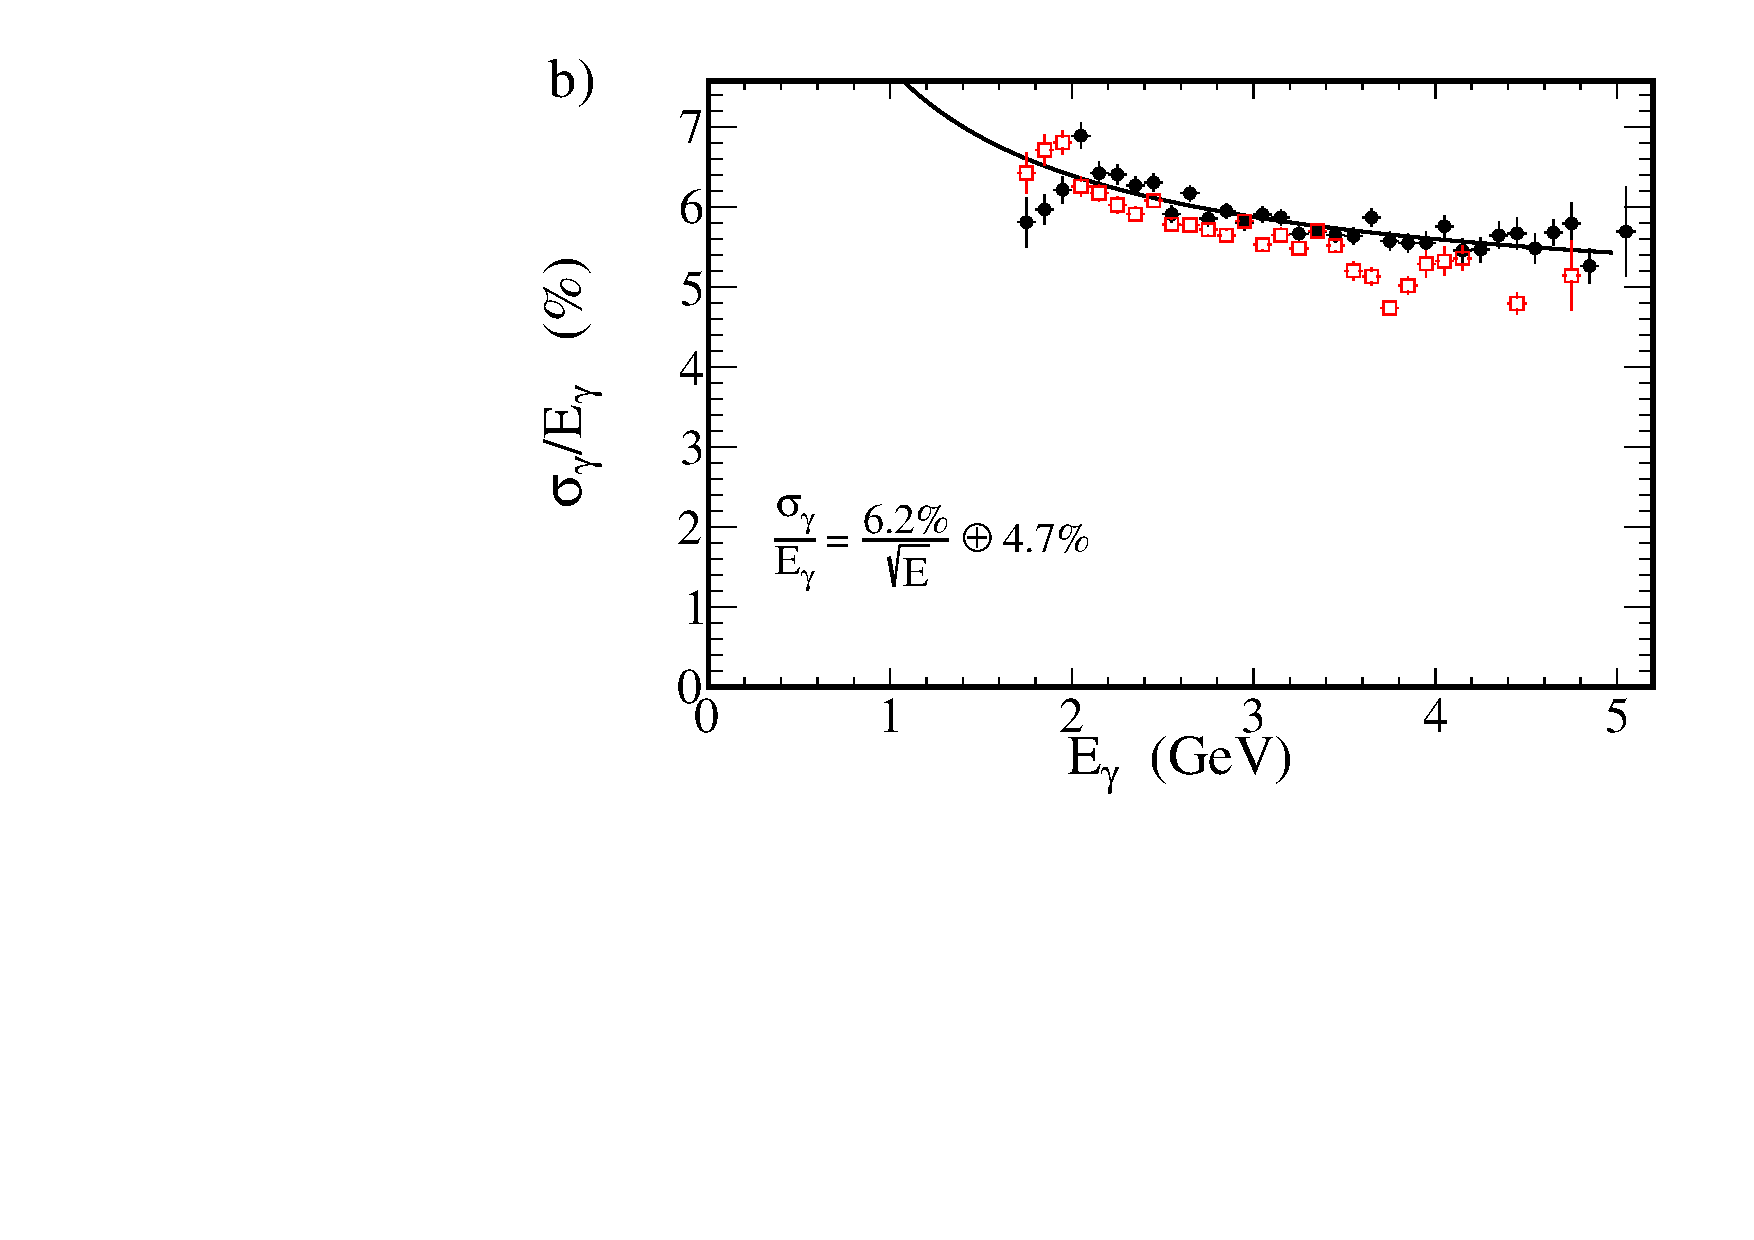
\includegraphics[width=0.48\textwidth]{figures/fit_FCAL_energy_resolution_sigma.pdf}
\caption{\label{fig:bcal:eta_resolution} 
The energy resolution of single photons in the a) BCAL and b) FCAL calculated from the $\eta$ mass distribution under the assumption that only the energy resolution contributes to its width.  Solid black circles are data and open red squares are simulation.
(Color online)
 }
\end{figure}    






\subsection{Summary \label{sec:calsummary}}